\section{Introduction}
\label{sec:introduction}
\IEEEPARstart{T}{inyTapeout} is a multi project chip platform that makes it easier and cheaper than ever to get ASIC designs manufactured.

Open source tools and process design kit (PDK~\cite{pdk}) are used, so no licenses or NDAs are needed. As the tools are run in the cloud, no software needs to be installed on the user's machine. However, as long as the template structure is followed, proprietary tools can be used.

Around 400 open source designs are multiplexed to 24 general purpose input/output (GPIO) pins, and after manufacture the chips are mounted to a demonstration board for easy testing. Each chip contains every design, which can be activated and tested in turn.

Additionally, each participant submits documentation for their design, collected to form a printable datasheet~\cite{datasheet} along with an online index at TinyTapeout.com/runs/~\cite{tinytapeoutruns}. The datasheet helps participants to explore each other's design in addition to their own.

By separating the cost of area and the physical chip, a group can share the cost of chip packaging and PCBs, while still getting to test and measure all the designs on the chip. In a classroom setting this helps to reduce the overall price, as students can share a smaller number of PCBs while each submitting their own design.

Each tile (Fig.~\ref{fig:render_cells_in_use}) is approximately $160 \times \qty{100}{\micro\meter\squared}$, enough for around 1000 logic gates on the Skywater 130nm open source PDK. Tiles can be joined to enable larger designs. Analog and mixed signal support is being added for the next shuttle.

Community engagement has been strong with 756 designs submitted over the first 5 shuttles. Some highlights are listed in section~\ref{sec:silicon_showcase}.
The online chat server has 1000 members with 1600 subscribed to the mailing list. Submitters tend to identify as hobbyists, students and teachers as shown in Fig.~\ref{fig:TT04_submitters}.

The first~\cite{firstshuttle} free and experimental shuttle with 152 designs was submitted to the seventh Google sponsored~\cite{googlesponsored} lottery multi project wafer (MPW) shuttle in September 2022.
The next 4 shuttles combined 582 designs and were sponsored by and manufactured with the Efabless~\cite{efabless} chipIgnite MPW service. Table~\ref{tab:tinytapeout} shows a summary of all the shuttle runs to date.

The rest of this paper will discuss the TinyTapeout design flow, multiplexer evolution, circuit boards, silicon results and next steps.

\begin{table*}[!t]
\centering
\caption{Statistics for Each of the TinyTapeout Shuttle Runs}
\label{tab:tinytapeout}
\begin{tabularx}{\textwidth}{@{}l *{8}{X}@{}}
\toprule
\textbf{Run} & \textbf{Launched} & \textbf{Shuttle} & \textbf{Designs} & \textbf{Delivery date} & \textbf{Architecture} & \textbf{Number of IOs} & \textbf{IO bandwidth} & \textbf{Analog support} \\
\midrule
TT01 & 2022-08-17  & MPW7  & 152 & n/a        & Scan chain                & 16 & \qty{5}{\kHz}    & no  \\
TT02 & 2022-11-09  & 2211Q & 165 & 2024-01-30 & Scan chain                & 16 & \qty{5}{\kHz}    & no  \\
TT03 & 2023-03-01  & 2304C & 249 & 2024-02-28 & Scan chain inverted clock & 16 & \qty{10}{\kHz}    & no  \\
TT04 & 2023-07-01  & 2309  & 143 & 2024-04-15 & Mux                       & 26 & \qty{50}{\MHz}   & no  \\
TT05 & 2023-09-11  & 2311  & 174 & 2024-05-12 & Split Mux                 & 26 & \qty{50}{\MHz}   & no  \\
TT06 & 2024-02-01  & 2404  & TBD & 2024-11-30 & Split Mux                 & 38 & \qty{50}{\MHz}   & yes \\
\bottomrule
\end{tabularx}
\end{table*}

\begin{figure}[!t]
\centering
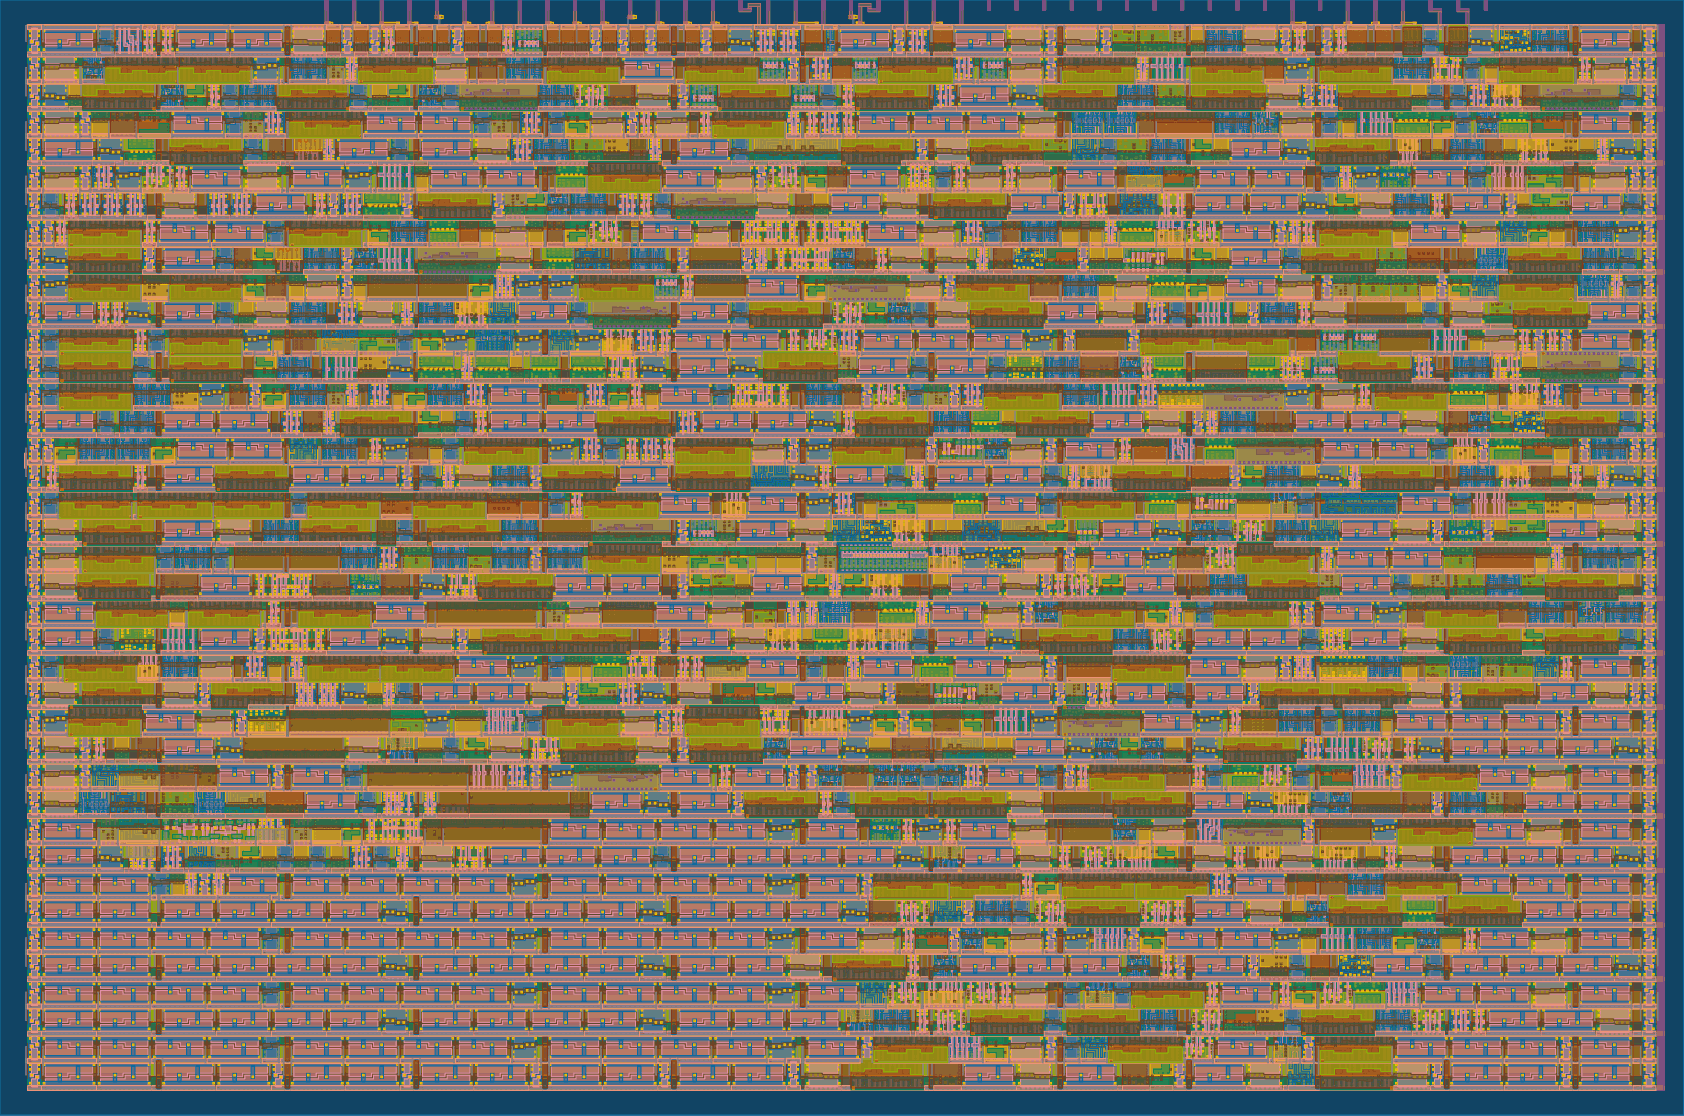
\includegraphics[width=\columnwidth]{./Figs/gh action gds layout.png}
\caption{2D render of a single tile}
\label{fig:render_cells_in_use}
\end{figure}

\begin{figure}[!t]
\centering
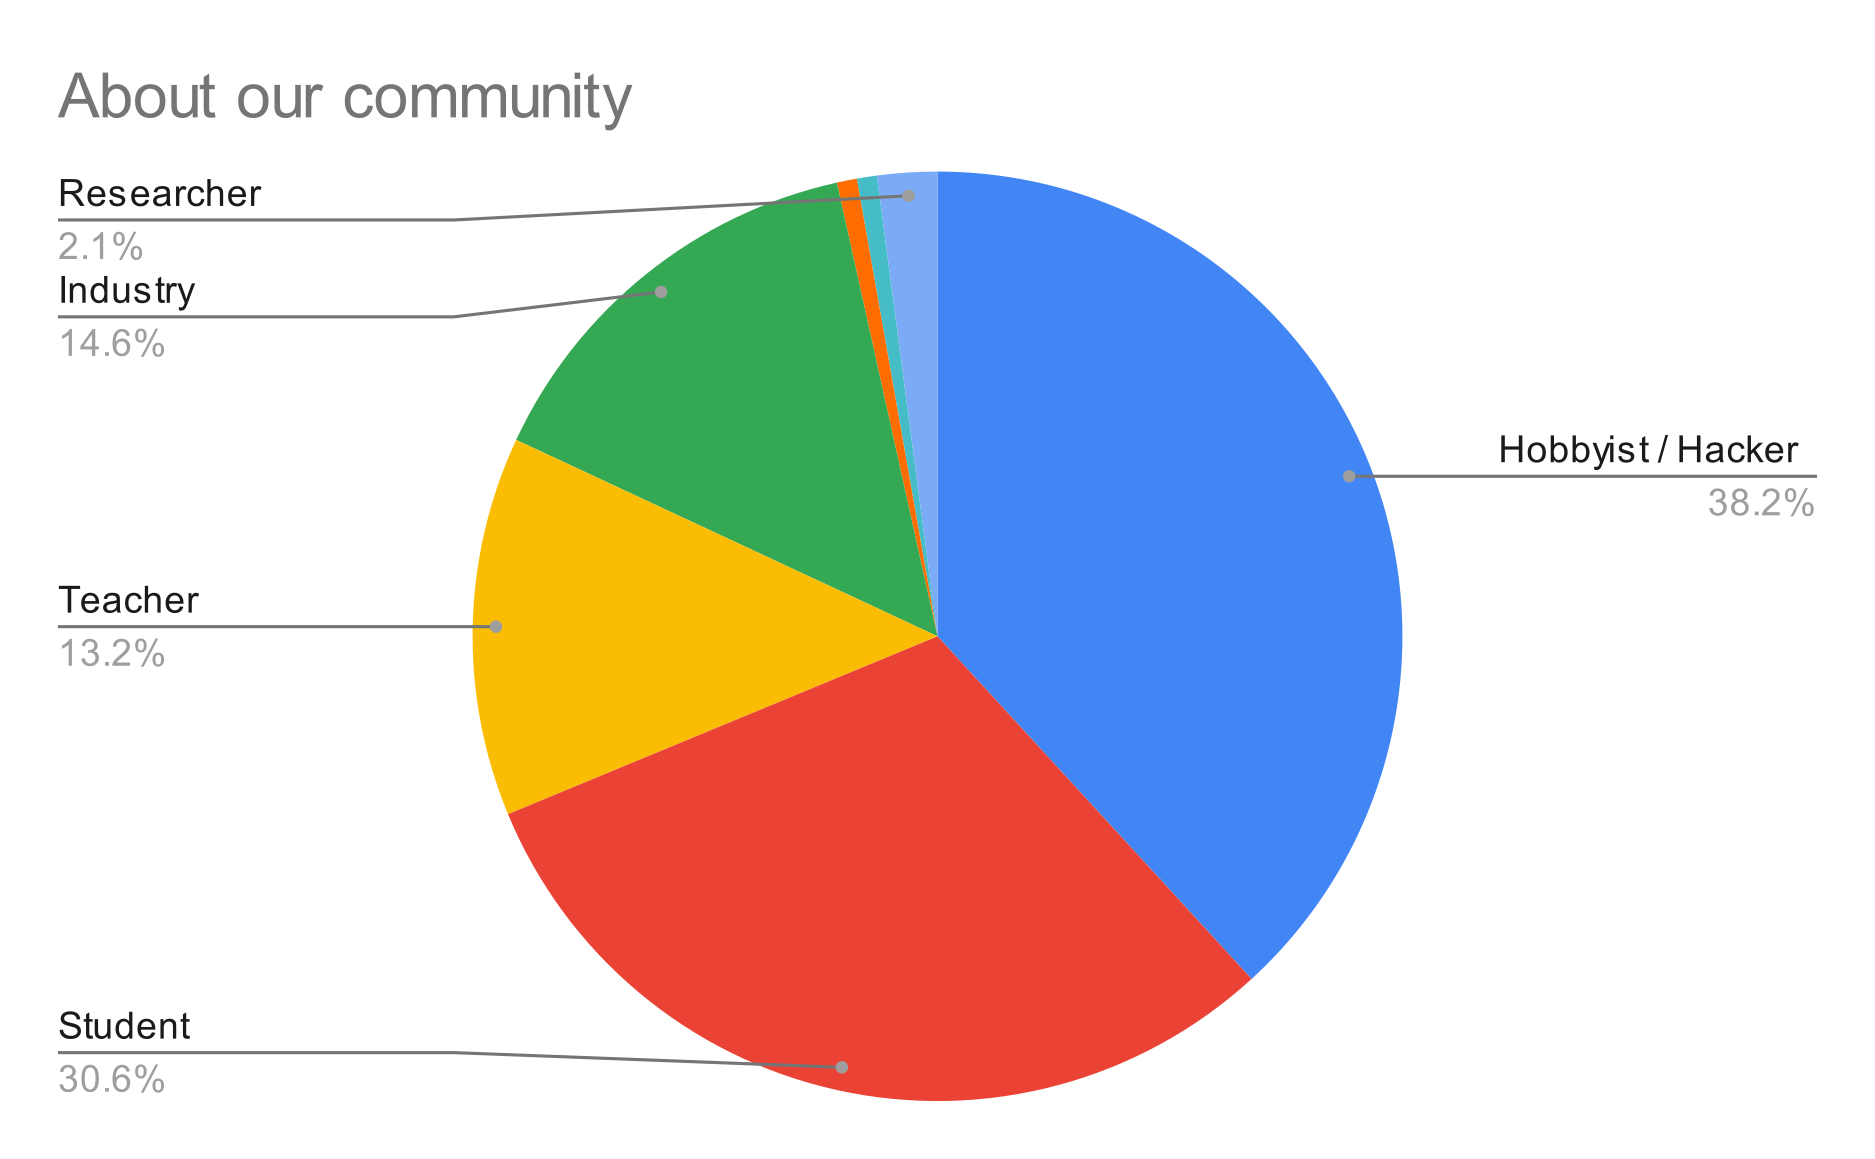
\includegraphics[width=\columnwidth]{./Figs/about our community pie chart.png}
\caption{How TT04 submitters identified themselves.}
\label{fig:TT04_submitters}
\end{figure}
